% Options for packages loaded elsewhere
\PassOptionsToPackage{unicode}{hyperref}
\PassOptionsToPackage{hyphens}{url}
%
\documentclass[
]{article}
\usepackage{amsmath,amssymb}
\usepackage{iftex}
\ifPDFTeX
  \usepackage[T1]{fontenc}
  \usepackage[utf8]{inputenc}
  \usepackage{textcomp} % provide euro and other symbols
\else % if luatex or xetex
  \usepackage{unicode-math} % this also loads fontspec
  \defaultfontfeatures{Scale=MatchLowercase}
  \defaultfontfeatures[\rmfamily]{Ligatures=TeX,Scale=1}
\fi
\usepackage{lmodern}
\ifPDFTeX\else
  % xetex/luatex font selection
\fi
% Use upquote if available, for straight quotes in verbatim environments
\IfFileExists{upquote.sty}{\usepackage{upquote}}{}
\IfFileExists{microtype.sty}{% use microtype if available
  \usepackage[]{microtype}
  \UseMicrotypeSet[protrusion]{basicmath} % disable protrusion for tt fonts
}{}
\makeatletter
\@ifundefined{KOMAClassName}{% if non-KOMA class
  \IfFileExists{parskip.sty}{%
    \usepackage{parskip}
  }{% else
    \setlength{\parindent}{0pt}
    \setlength{\parskip}{6pt plus 2pt minus 1pt}}
}{% if KOMA class
  \KOMAoptions{parskip=half}}
\makeatother
\usepackage{xcolor}
\usepackage[margin=1in]{geometry}
\usepackage{color}
\usepackage{fancyvrb}
\newcommand{\VerbBar}{|}
\newcommand{\VERB}{\Verb[commandchars=\\\{\}]}
\DefineVerbatimEnvironment{Highlighting}{Verbatim}{commandchars=\\\{\}}
% Add ',fontsize=\small' for more characters per line
\usepackage{framed}
\definecolor{shadecolor}{RGB}{248,248,248}
\newenvironment{Shaded}{\begin{snugshade}}{\end{snugshade}}
\newcommand{\AlertTok}[1]{\textcolor[rgb]{0.94,0.16,0.16}{#1}}
\newcommand{\AnnotationTok}[1]{\textcolor[rgb]{0.56,0.35,0.01}{\textbf{\textit{#1}}}}
\newcommand{\AttributeTok}[1]{\textcolor[rgb]{0.13,0.29,0.53}{#1}}
\newcommand{\BaseNTok}[1]{\textcolor[rgb]{0.00,0.00,0.81}{#1}}
\newcommand{\BuiltInTok}[1]{#1}
\newcommand{\CharTok}[1]{\textcolor[rgb]{0.31,0.60,0.02}{#1}}
\newcommand{\CommentTok}[1]{\textcolor[rgb]{0.56,0.35,0.01}{\textit{#1}}}
\newcommand{\CommentVarTok}[1]{\textcolor[rgb]{0.56,0.35,0.01}{\textbf{\textit{#1}}}}
\newcommand{\ConstantTok}[1]{\textcolor[rgb]{0.56,0.35,0.01}{#1}}
\newcommand{\ControlFlowTok}[1]{\textcolor[rgb]{0.13,0.29,0.53}{\textbf{#1}}}
\newcommand{\DataTypeTok}[1]{\textcolor[rgb]{0.13,0.29,0.53}{#1}}
\newcommand{\DecValTok}[1]{\textcolor[rgb]{0.00,0.00,0.81}{#1}}
\newcommand{\DocumentationTok}[1]{\textcolor[rgb]{0.56,0.35,0.01}{\textbf{\textit{#1}}}}
\newcommand{\ErrorTok}[1]{\textcolor[rgb]{0.64,0.00,0.00}{\textbf{#1}}}
\newcommand{\ExtensionTok}[1]{#1}
\newcommand{\FloatTok}[1]{\textcolor[rgb]{0.00,0.00,0.81}{#1}}
\newcommand{\FunctionTok}[1]{\textcolor[rgb]{0.13,0.29,0.53}{\textbf{#1}}}
\newcommand{\ImportTok}[1]{#1}
\newcommand{\InformationTok}[1]{\textcolor[rgb]{0.56,0.35,0.01}{\textbf{\textit{#1}}}}
\newcommand{\KeywordTok}[1]{\textcolor[rgb]{0.13,0.29,0.53}{\textbf{#1}}}
\newcommand{\NormalTok}[1]{#1}
\newcommand{\OperatorTok}[1]{\textcolor[rgb]{0.81,0.36,0.00}{\textbf{#1}}}
\newcommand{\OtherTok}[1]{\textcolor[rgb]{0.56,0.35,0.01}{#1}}
\newcommand{\PreprocessorTok}[1]{\textcolor[rgb]{0.56,0.35,0.01}{\textit{#1}}}
\newcommand{\RegionMarkerTok}[1]{#1}
\newcommand{\SpecialCharTok}[1]{\textcolor[rgb]{0.81,0.36,0.00}{\textbf{#1}}}
\newcommand{\SpecialStringTok}[1]{\textcolor[rgb]{0.31,0.60,0.02}{#1}}
\newcommand{\StringTok}[1]{\textcolor[rgb]{0.31,0.60,0.02}{#1}}
\newcommand{\VariableTok}[1]{\textcolor[rgb]{0.00,0.00,0.00}{#1}}
\newcommand{\VerbatimStringTok}[1]{\textcolor[rgb]{0.31,0.60,0.02}{#1}}
\newcommand{\WarningTok}[1]{\textcolor[rgb]{0.56,0.35,0.01}{\textbf{\textit{#1}}}}
\usepackage{longtable,booktabs,array}
\usepackage{calc} % for calculating minipage widths
% Correct order of tables after \paragraph or \subparagraph
\usepackage{etoolbox}
\makeatletter
\patchcmd\longtable{\par}{\if@noskipsec\mbox{}\fi\par}{}{}
\makeatother
% Allow footnotes in longtable head/foot
\IfFileExists{footnotehyper.sty}{\usepackage{footnotehyper}}{\usepackage{footnote}}
\makesavenoteenv{longtable}
\usepackage{graphicx}
\makeatletter
\def\maxwidth{\ifdim\Gin@nat@width>\linewidth\linewidth\else\Gin@nat@width\fi}
\def\maxheight{\ifdim\Gin@nat@height>\textheight\textheight\else\Gin@nat@height\fi}
\makeatother
% Scale images if necessary, so that they will not overflow the page
% margins by default, and it is still possible to overwrite the defaults
% using explicit options in \includegraphics[width, height, ...]{}
\setkeys{Gin}{width=\maxwidth,height=\maxheight,keepaspectratio}
% Set default figure placement to htbp
\makeatletter
\def\fps@figure{htbp}
\makeatother
\setlength{\emergencystretch}{3em} % prevent overfull lines
\providecommand{\tightlist}{%
  \setlength{\itemsep}{0pt}\setlength{\parskip}{0pt}}
\setcounter{secnumdepth}{-\maxdimen} % remove section numbering
\ifLuaTeX
  \usepackage{selnolig}  % disable illegal ligatures
\fi
\IfFileExists{bookmark.sty}{\usepackage{bookmark}}{\usepackage{hyperref}}
\IfFileExists{xurl.sty}{\usepackage{xurl}}{} % add URL line breaks if available
\urlstyle{same}
\hypersetup{
  pdftitle={OJ-Purchase-Prediction},
  pdfauthor={Nikhil Prema Chandra Rao},
  hidelinks,
  pdfcreator={LaTeX via pandoc}}

\title{OJ-Purchase-Prediction}
\author{Nikhil Prema Chandra Rao}
\date{2024-10-27}

\begin{document}
\maketitle

\hypertarget{introduction}{%
\section{Introduction}\label{introduction}}

In this analysis, we aim to predict whether a customer will purchase
\textbf{Citrus Hill} or \textbf{Minute Maid} orange juice using the
\textbf{OJ} data set from the \texttt{ISLR2} library. We will develop a
\textbf{Decision Tree} model and explore its accuracy in predicting
customer purchases. We will also visualize the decision-making process,
inspect feature importance, and improve the model through hyper
parameter tuning. The goal is to provide a comprehensive, step-by-step
explanation using R code and visualizations.

\hypertarget{data-loading-and-preprocessing}{%
\subsection{Data Loading and
Preprocessing}\label{data-loading-and-preprocessing}}

\begin{Shaded}
\begin{Highlighting}[]
\FunctionTok{library}\NormalTok{(ISLR2)}
\FunctionTok{library}\NormalTok{(caret)}
\end{Highlighting}
\end{Shaded}

\begin{verbatim}
## Loading required package: ggplot2
\end{verbatim}

\begin{verbatim}
## Loading required package: lattice
\end{verbatim}

\begin{Shaded}
\begin{Highlighting}[]
\FunctionTok{library}\NormalTok{(rpart)}
\FunctionTok{library}\NormalTok{(rpart.plot)}
\FunctionTok{library}\NormalTok{(ggplot2)}
\FunctionTok{library}\NormalTok{(dplyr)}
\end{Highlighting}
\end{Shaded}

\begin{verbatim}
## 
## Attaching package: 'dplyr'
\end{verbatim}

\begin{verbatim}
## The following objects are masked from 'package:stats':
## 
##     filter, lag
\end{verbatim}

\begin{verbatim}
## The following objects are masked from 'package:base':
## 
##     intersect, setdiff, setequal, union
\end{verbatim}

\begin{Shaded}
\begin{Highlighting}[]
\FunctionTok{data}\NormalTok{(OJ)}

\FunctionTok{sum}\NormalTok{(}\FunctionTok{is.na}\NormalTok{(OJ))}
\end{Highlighting}
\end{Shaded}

\begin{verbatim}
## [1] 0
\end{verbatim}

\begin{Shaded}
\begin{Highlighting}[]
\FunctionTok{str}\NormalTok{(OJ)}
\end{Highlighting}
\end{Shaded}

\begin{verbatim}
## 'data.frame':    1070 obs. of  18 variables:
##  $ Purchase      : Factor w/ 2 levels "CH","MM": 1 1 1 2 1 1 1 1 1 1 ...
##  $ WeekofPurchase: num  237 239 245 227 228 230 232 234 235 238 ...
##  $ StoreID       : num  1 1 1 1 7 7 7 7 7 7 ...
##  $ PriceCH       : num  1.75 1.75 1.86 1.69 1.69 1.69 1.69 1.75 1.75 1.75 ...
##  $ PriceMM       : num  1.99 1.99 2.09 1.69 1.69 1.99 1.99 1.99 1.99 1.99 ...
##  $ DiscCH        : num  0 0 0.17 0 0 0 0 0 0 0 ...
##  $ DiscMM        : num  0 0.3 0 0 0 0 0.4 0.4 0.4 0.4 ...
##  $ SpecialCH     : num  0 0 0 0 0 0 1 1 0 0 ...
##  $ SpecialMM     : num  0 1 0 0 0 1 1 0 0 0 ...
##  $ LoyalCH       : num  0.5 0.6 0.68 0.4 0.957 ...
##  $ SalePriceMM   : num  1.99 1.69 2.09 1.69 1.69 1.99 1.59 1.59 1.59 1.59 ...
##  $ SalePriceCH   : num  1.75 1.75 1.69 1.69 1.69 1.69 1.69 1.75 1.75 1.75 ...
##  $ PriceDiff     : num  0.24 -0.06 0.4 0 0 0.3 -0.1 -0.16 -0.16 -0.16 ...
##  $ Store7        : Factor w/ 2 levels "No","Yes": 1 1 1 1 2 2 2 2 2 2 ...
##  $ PctDiscMM     : num  0 0.151 0 0 0 ...
##  $ PctDiscCH     : num  0 0 0.0914 0 0 ...
##  $ ListPriceDiff : num  0.24 0.24 0.23 0 0 0.3 0.3 0.24 0.24 0.24 ...
##  $ STORE         : num  1 1 1 1 0 0 0 0 0 0 ...
\end{verbatim}

\begin{Shaded}
\begin{Highlighting}[]
\NormalTok{OJ}\SpecialCharTok{$}\NormalTok{Purchase }\OtherTok{\textless{}{-}} \FunctionTok{as.factor}\NormalTok{(OJ}\SpecialCharTok{$}\NormalTok{Purchase)}
\end{Highlighting}
\end{Shaded}

In this section, we load the necessary libraries such as ISLR2 (for the
data set), caret (for data partitioning and model tuning), rpart (for
decision tree modeling), and ggplot2 for data visualization. This
dataset contains 1,070 observations and 18 variables related to
purchases of two products, CH and MM, across different stores. The
variables include details such as the week of purchase, store ID, and
pricing information for both products, including discount rates, special
offers, and loyalty metrics. Additionally, it provides computed fields
like the price difference between the products and sale prices. The data
is structured to facilitate analysis of purchasing patterns and factors
influencing consumer choice between CH and MM.

We check for any missing values in the data set and convert the response
variable Purchase into a factor, which is essential for classification
tasks.

\hypertarget{data-splitting}{%
\subsection{Data Splitting}\label{data-splitting}}

To evaluate the model, we split the data set into training and testing
sets. This ensures that the model is trained on one subset of the data
and then tested on unseen data for an unbiased evaluation.

\begin{Shaded}
\begin{Highlighting}[]
\FunctionTok{set.seed}\NormalTok{(}\DecValTok{123}\NormalTok{)}
\NormalTok{train\_index }\OtherTok{\textless{}{-}} \FunctionTok{createDataPartition}\NormalTok{(OJ}\SpecialCharTok{$}\NormalTok{Purchase, }\AttributeTok{p =} \FloatTok{0.7}\NormalTok{, }\AttributeTok{list =} \ConstantTok{FALSE}\NormalTok{)}
\NormalTok{train\_data }\OtherTok{\textless{}{-}}\NormalTok{ OJ[train\_index, ]}
\NormalTok{test\_data }\OtherTok{\textless{}{-}}\NormalTok{ OJ[}\SpecialCharTok{{-}}\NormalTok{train\_index, ]}
\end{Highlighting}
\end{Shaded}

\hypertarget{exploratory-data-analysis-eda}{%
\subsection{Exploratory Data Analysis
(EDA)}\label{exploratory-data-analysis-eda}}

\hypertarget{distribution-of-purchases}{%
\subsubsection{Distribution of
Purchases}\label{distribution-of-purchases}}

\begin{Shaded}
\begin{Highlighting}[]
\FunctionTok{ggplot}\NormalTok{(OJ, }\FunctionTok{aes}\NormalTok{(}\AttributeTok{x =}\NormalTok{ Purchase)) }\SpecialCharTok{+}
  \FunctionTok{geom\_bar}\NormalTok{(}\AttributeTok{fill =} \StringTok{"lightblue"}\NormalTok{) }\SpecialCharTok{+}
  \FunctionTok{ggtitle}\NormalTok{(}\StringTok{"Distribution of Purchase (Citrus Hill vs. Minute Maid)"}\NormalTok{) }\SpecialCharTok{+}
  \FunctionTok{xlab}\NormalTok{(}\StringTok{"Purchase"}\NormalTok{) }\SpecialCharTok{+} \FunctionTok{ylab}\NormalTok{(}\StringTok{"Count"}\NormalTok{)}
\end{Highlighting}
\end{Shaded}

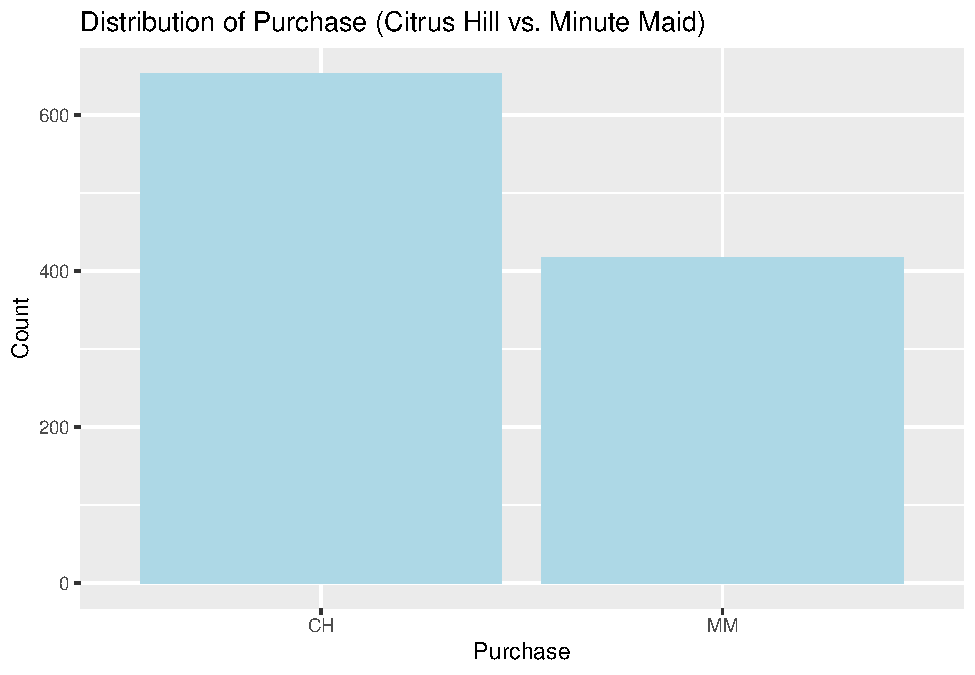
\includegraphics{OJ_files/figure-latex/unnamed-chunk-3-1.pdf}

This bar plot shows the distribution of purchases between Citrus Hill
and Minute Maid. It helps us understand the balance of the response
variable, which is important when building classification models. The
bar chart displays the distribution of purchases between Citrus Hill
(CH) and Minute Maid (MM) orange juice. The taller bar for Citrus Hill
indicates that it is purchased more frequently than Minute Maid in the
dataset, with over 600 purchases for CH compared to around 400 for MM.
This imbalance suggests that Citrus Hill is the more popular choice
overall.

\hypertarget{scatter-plot-price-of-citrus-hill-vs.-minute-maid}{%
\subsubsection{Scatter Plot: Price of Citrus Hill vs.~Minute
Maid}\label{scatter-plot-price-of-citrus-hill-vs.-minute-maid}}

\begin{Shaded}
\begin{Highlighting}[]
\FunctionTok{ggplot}\NormalTok{(OJ, }\FunctionTok{aes}\NormalTok{(}\AttributeTok{x =}\NormalTok{ PriceCH, }\AttributeTok{y =}\NormalTok{ PriceMM, }\AttributeTok{color =}\NormalTok{ Purchase)) }\SpecialCharTok{+}
  \FunctionTok{geom\_point}\NormalTok{(}\AttributeTok{alpha =} \FloatTok{0.6}\NormalTok{) }\SpecialCharTok{+}
  \FunctionTok{ggtitle}\NormalTok{(}\StringTok{"Price of Citrus Hill vs. Price of Minute Maid by Purchase"}\NormalTok{) }\SpecialCharTok{+}
  \FunctionTok{xlab}\NormalTok{(}\StringTok{"Price of Citrus Hill"}\NormalTok{) }\SpecialCharTok{+} \FunctionTok{ylab}\NormalTok{(}\StringTok{"Price of Minute Maid"}\NormalTok{)}
\end{Highlighting}
\end{Shaded}

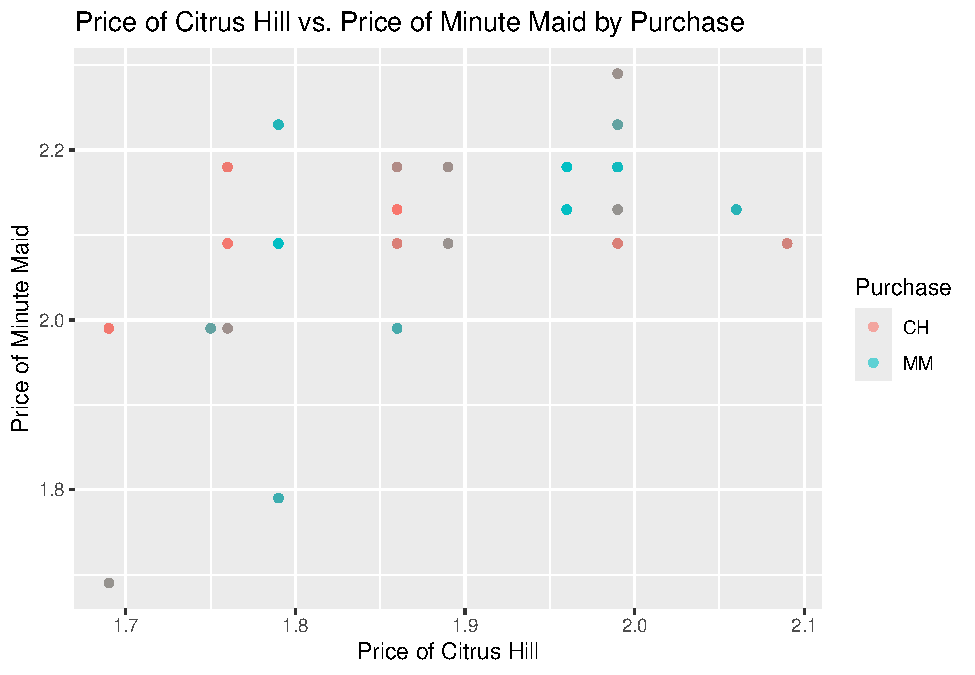
\includegraphics{OJ_files/figure-latex/unnamed-chunk-4-1.pdf}

In this scatter plot, we compare the prices of Citrus Hill and Minute
Maid with respect to the purchases. Points are colored by Purchase,
allowing us to see the relationship between the prices and the purchase
decision. The scatter plot visualizes the relationship between the
prices of Citrus Hill (x-axis) and Minute Maid (y-axis) for different
purchase decisions. Points are color-coded by the product purchased (CH
or MM). There is some overlap between the two products, but it is
evident that lower prices for one product might influence the decision
to purchase the other.

\hypertarget{density-plots-price-of-citrus-hill-vs.-price-of-minute-maid-by-purchase}{%
\subsubsection{Density Plots: Price of Citrus Hill vs.~Price of Minute
Maid by
Purchase}\label{density-plots-price-of-citrus-hill-vs.-price-of-minute-maid-by-purchase}}

\begin{Shaded}
\begin{Highlighting}[]
\FunctionTok{ggplot}\NormalTok{(OJ, }\FunctionTok{aes}\NormalTok{(}\AttributeTok{x =}\NormalTok{ PriceCH, }\AttributeTok{fill =}\NormalTok{ Purchase)) }\SpecialCharTok{+}
  \FunctionTok{geom\_density}\NormalTok{(}\AttributeTok{alpha =} \FloatTok{0.4}\NormalTok{) }\SpecialCharTok{+}
  \FunctionTok{ggtitle}\NormalTok{(}\StringTok{"Distribution of Price for Citrus Hill by Purchase"}\NormalTok{) }\SpecialCharTok{+}
  \FunctionTok{xlab}\NormalTok{(}\StringTok{"Price of Citrus Hill"}\NormalTok{)}
\end{Highlighting}
\end{Shaded}

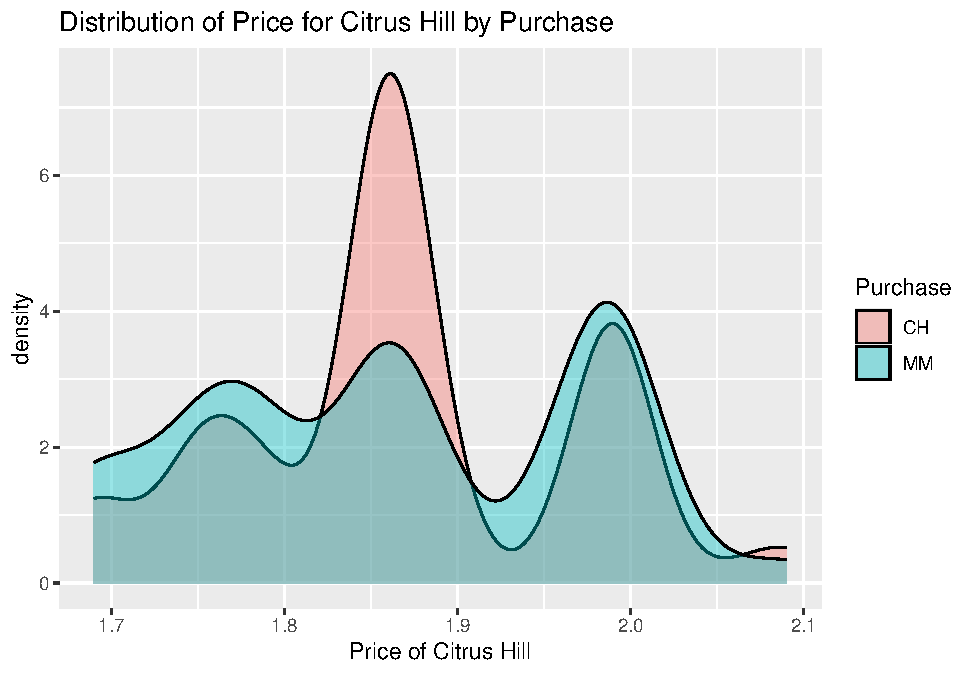
\includegraphics{OJ_files/figure-latex/unnamed-chunk-5-1.pdf}

The density plot shows the distribution of prices for Citrus Hill (CH),
separated by the product purchased (either Citrus Hill (CH) or Minute
Maid (MM)), using different colors. The x-axis represents the price of
Citrus Hill, while the y-axis indicates the density, or the relative
frequency of different prices in the dataset.

\begin{itemize}
\tightlist
\item
  The red area represents customers who purchased Citrus Hill at various
  price points, and the teal area represents those who purchased Minute
  Maid.
\item
  The peak for Citrus Hill purchases (red) occurs around a price of 1.9,
  indicating that customers tend to buy Citrus Hill more frequently at
  this price range.
\item
  Minute Maid purchases (teal) are more spread out, with some preference
  for lower prices of Citrus Hill (1.7 to 1.8) and higher prices (around
  2.0), possibly indicating that when Citrus Hill is priced low or high,
  more customers opt for Minute Maid. This visualization helps to
  understand how the pricing of Citrus Hill influences whether customers
  purchase it or opt for its competitor.
\end{itemize}

\hypertarget{density-plots-price-for-minute-maid-by-purchase}{%
\subsubsection{Density Plots: Price for minute maid by
purchase}\label{density-plots-price-for-minute-maid-by-purchase}}

\begin{Shaded}
\begin{Highlighting}[]
\FunctionTok{ggplot}\NormalTok{(OJ, }\FunctionTok{aes}\NormalTok{(}\AttributeTok{x =}\NormalTok{ PriceMM, }\AttributeTok{fill =}\NormalTok{ Purchase)) }\SpecialCharTok{+}
  \FunctionTok{geom\_density}\NormalTok{(}\AttributeTok{alpha =} \FloatTok{0.4}\NormalTok{) }\SpecialCharTok{+}
  \FunctionTok{ggtitle}\NormalTok{(}\StringTok{"Distribution of Price for Minute Maid by Purchase"}\NormalTok{) }\SpecialCharTok{+}
  \FunctionTok{xlab}\NormalTok{(}\StringTok{"Price of Minute Maid"}\NormalTok{)}
\end{Highlighting}
\end{Shaded}

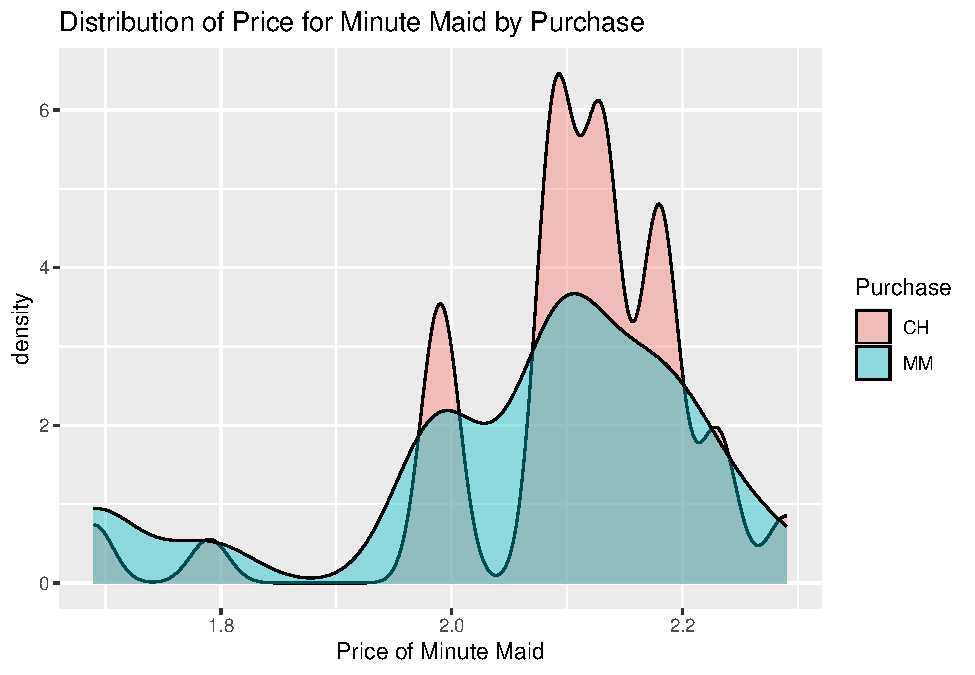
\includegraphics{OJ_files/figure-latex/unnamed-chunk-6-1.pdf}

This density plot shows the price distribution of Minute Maid purchases
by two groups: CH (red) and MM (blue). Both groups frequently buy around
the 2.0--2.2 price range, with CH purchases being more concentrated
around specific price points (2.0 and 2.1). MM purchases have a wider
spread, including some lower prices (around 1.7), indicating more
variability in purchase prices compared to CH. The overlap suggests
shared popular price points, but MM appears more price-flexible.

\hypertarget{building-the-initial-decision-tree-model}{%
\subsection{Building the Initial Decision Tree
Model}\label{building-the-initial-decision-tree-model}}

\begin{Shaded}
\begin{Highlighting}[]
\NormalTok{tree\_model }\OtherTok{\textless{}{-}} \FunctionTok{rpart}\NormalTok{(Purchase }\SpecialCharTok{\textasciitilde{}}\NormalTok{ ., }\AttributeTok{data =}\NormalTok{ train\_data, }\AttributeTok{method =} \StringTok{"class"}\NormalTok{)}

\FunctionTok{rpart.plot}\NormalTok{(tree\_model, }\AttributeTok{type =} \DecValTok{3}\NormalTok{, }\AttributeTok{extra =} \DecValTok{102}\NormalTok{, }\AttributeTok{under =} \ConstantTok{TRUE}\NormalTok{, }\AttributeTok{fallen.leaves =} \ConstantTok{TRUE}\NormalTok{)}
\end{Highlighting}
\end{Shaded}

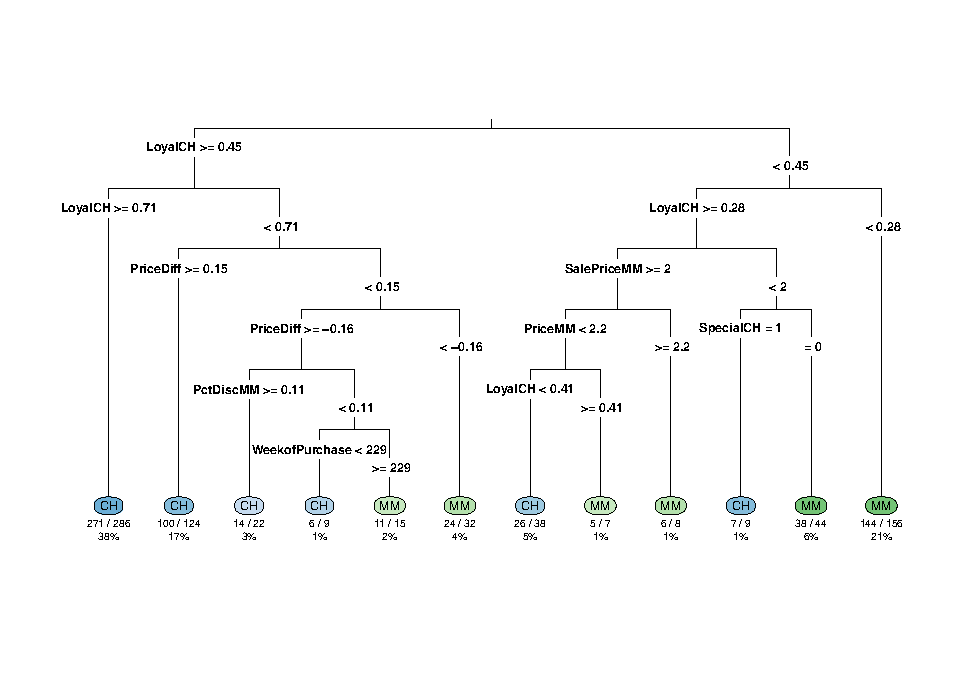
\includegraphics{OJ_files/figure-latex/unnamed-chunk-7-1.pdf}

The Decision Tree is built using the rpart function. A Decision Tree
works by splitting the data at each node based on the feature that best
separates the classes (Citrus Hill and Minute Maid) using criteria like
Gini Impurity. The resulting tree is plotted to visualize how the
features (e.g., prices, demographics) are used to make predictions at
each step. Interpretation of the Tree

\begin{itemize}
\tightlist
\item
  \textbf{Nodes}: Each internal node represents a decision rule based on
  a feature.
\item
  \textbf{Branches}: Each branch represents the outcome of the decision
  (true or false).
\item
  \textbf{Leaves}: The terminal nodes (leaves) display the predicted
  class for the samples that reach them.
\end{itemize}

This decision tree classifies customers into two categories, ``CH'' and
``MM,'' based primarily on the \texttt{LoyalCH} feature, which likely
represents a customer loyalty score. At the root, if \texttt{LoyalCH} is
0.45 or higher, the tree branches left; otherwise, it goes right. For
customers with a high \texttt{LoyalCH} (≥ 0.71), the next decision
depends on \texttt{PriceDiff}. If \texttt{PriceDiff} is 0.15 or more,
the classification is ``CH''; if it's lower, further splits occur based
on \texttt{PctDiscMM} (percentage discount) and \texttt{WeekofPurchase}.
If \texttt{LoyalCH} is between 0.45 and 0.71, additional splits occur
using \texttt{PriceMM}, \texttt{LoyalCH}, and \texttt{SalePriceMM} until
a final decision is reached.

For customers with \texttt{LoyalCH} below 0.45, the tree uses
\texttt{LoyalCH} thresholds at 0.28 and conditions based on
\texttt{SalePriceMM} and \texttt{SpecialCH} to make classifications.
Each endpoint represents a final classification into ``CH'' or ``MM,''
showing the number and percentage of instances in that category. This
structure indicates that \texttt{LoyalCH} is a crucial determinant in
the model, influencing classification outcomes across both high and low
loyalty levels.

\hypertarget{evaluating-the-model}{%
\subsection{Evaluating the Model}\label{evaluating-the-model}}

\begin{Shaded}
\begin{Highlighting}[]
\NormalTok{test\_pred }\OtherTok{\textless{}{-}} \FunctionTok{predict}\NormalTok{(tree\_model, }\AttributeTok{newdata =}\NormalTok{ test\_data, }\AttributeTok{type =} \StringTok{"class"}\NormalTok{)}
\FunctionTok{confusionMatrix}\NormalTok{(test\_pred, test\_data}\SpecialCharTok{$}\NormalTok{Purchase)}
\end{Highlighting}
\end{Shaded}

\begin{verbatim}
## Confusion Matrix and Statistics
## 
##           Reference
## Prediction  CH  MM
##         CH 169  33
##         MM  26  92
##                                           
##                Accuracy : 0.8156          
##                  95% CI : (0.7687, 0.8566)
##     No Information Rate : 0.6094          
##     P-Value [Acc > NIR] : 1.373e-15       
##                                           
##                   Kappa : 0.6088          
##                                           
##  Mcnemar's Test P-Value : 0.4347          
##                                           
##             Sensitivity : 0.8667          
##             Specificity : 0.7360          
##          Pos Pred Value : 0.8366          
##          Neg Pred Value : 0.7797          
##              Prevalence : 0.6094          
##          Detection Rate : 0.5281          
##    Detection Prevalence : 0.6312          
##       Balanced Accuracy : 0.8013          
##                                           
##        'Positive' Class : CH              
## 
\end{verbatim}

\begin{Shaded}
\begin{Highlighting}[]
\NormalTok{initial\_accuracy }\OtherTok{\textless{}{-}} \FunctionTok{sum}\NormalTok{(test\_pred }\SpecialCharTok{==}\NormalTok{ test\_data}\SpecialCharTok{$}\NormalTok{Purchase) }\SpecialCharTok{/} \FunctionTok{nrow}\NormalTok{(test\_data)}
\FunctionTok{print}\NormalTok{(}\FunctionTok{paste}\NormalTok{(}\StringTok{"Initial Accuracy:"}\NormalTok{, }\FunctionTok{round}\NormalTok{(initial\_accuracy }\SpecialCharTok{*} \DecValTok{100}\NormalTok{, }\DecValTok{2}\NormalTok{), }\StringTok{"\%"}\NormalTok{))}
\end{Highlighting}
\end{Shaded}

\begin{verbatim}
## [1] "Initial Accuracy: 81.56 %"
\end{verbatim}

Explanation:

\hypertarget{confusion-matrix-overview}{%
\subsubsection{\texorpdfstring{1. \textbf{Confusion Matrix
Overview}}{1. Confusion Matrix Overview}}\label{confusion-matrix-overview}}

The confusion matrix presents a summary of the prediction results of a
classification model. In this case, you have two classes: \textbf{CH}
(presumably representing one category) and \textbf{MM} (representing
another category). The matrix is structured as follows:

\begin{longtable}[]{@{}lll@{}}
\toprule\noalign{}
& Reference CH & Reference MM \\
\midrule\noalign{}
\endhead
\bottomrule\noalign{}
\endlastfoot
\textbf{Predicted CH} & 169 & 33 \\
\textbf{Predicted MM} & 26 & 92 \\
\end{longtable}

\textbf{Interpretation:} - \textbf{True Positives (TP)}: 169 instances
were correctly predicted as CH. - \textbf{False Negatives (FN)}: 33
instances were incorrectly predicted as MM when they were actually CH. -
\textbf{False Positives (FP)}: 26 instances were incorrectly predicted
as CH when they were actually MM. - \textbf{True Negatives (TN)}: 92
instances were correctly predicted as MM.

\hypertarget{model-performance-metrics}{%
\subsubsection{\texorpdfstring{2. \textbf{Model Performance
Metrics}}{2. Model Performance Metrics}}\label{model-performance-metrics}}

\textbf{Accuracy}: The proportion of correct predictions (both true
positives and true negatives) among the total predictions.

\begin{itemize}
\tightlist
\item
  \textbf{Calculation}: \[
  \text{Accuracy} = \frac{TP + TN}{TP + TN + FP + FN} = \frac{169 + 92}{169 + 33 + 26 + 92} = 0.8156 \text{ or } 81.56\%
  \]
\item
  \textbf{Interpretation}: About 81.56\% of the total predictions made
  by the model were correct.
\end{itemize}

\textbf{95\% Confidence Interval (CI)}: - \textbf{Interpretation}: This
interval (0.7687, 0.8566) indicates that we can be 95\% confident that
the true accuracy of the model lies within this range.

\textbf{No Information Rate (NIR)}: The accuracy expected if predictions
were made solely based on the most frequent class (in this case, CH). -
\textbf{Value}: 0.6094 indicates that if you simply predicted the most
common class, you would be correct about 60.94\% of the time.

\textbf{P-Value {[}Acc \textgreater{} NIR{]}}: - \textbf{Value}:
1.373e-15 indicates that the model's accuracy is significantly better
than the no information rate, suggesting that the model is effective.

\hypertarget{kappa-statistic}{%
\subsubsection{\texorpdfstring{3. \textbf{Kappa
Statistic}}{3. Kappa Statistic}}\label{kappa-statistic}}

Kappa measures the agreement between the predicted and actual
classifications, correcting for chance. - \textbf{Value}: 0.6088,
indicating a moderate level of agreement beyond chance. Values closer to
1 imply better agreement.

\hypertarget{mcnemars-test-p-value}{%
\subsubsection{\texorpdfstring{4. \textbf{Mcnemar's Test
P-Value}}{4. Mcnemar's Test P-Value}}\label{mcnemars-test-p-value}}

\begin{itemize}
\tightlist
\item
  \textbf{Value}: 0.4347 indicates no significant difference in the
  error rates of the two classes, suggesting that the model does not
  favor one class over the other.
\end{itemize}

\hypertarget{sensitivity-true-positive-rate}{%
\subsubsection{\texorpdfstring{5. \textbf{Sensitivity (True Positive
Rate)}}{5. Sensitivity (True Positive Rate)}}\label{sensitivity-true-positive-rate}}

The proportion of actual positives that are correctly identified. -
\textbf{Calculation}: \[
  \text{Sensitivity} = \frac{TP}{TP + FN} = \frac{169}{169 + 33} = 0.8667 \text{ or } 86.67\%
  \] - \textbf{Interpretation}: The model correctly identifies 86.67\%
of actual CH instances.

\hypertarget{specificity-true-negative-rate}{%
\subsubsection{\texorpdfstring{6. \textbf{Specificity (True Negative
Rate)}}{6. Specificity (True Negative Rate)}}\label{specificity-true-negative-rate}}

The proportion of actual negatives that are correctly identified. -
\textbf{Calculation}: \[
  \text{Specificity} = \frac{TN}{TN + FP} = \frac{92}{92 + 26} = 0.7360 \text{ or } 73.60\%
  \] - \textbf{Interpretation}: The model correctly identifies 73.60\%
of actual MM instances.

\hypertarget{positive-predictive-value-ppv}{%
\subsubsection{\texorpdfstring{7. \textbf{Positive Predictive Value
(PPV)}}{7. Positive Predictive Value (PPV)}}\label{positive-predictive-value-ppv}}

The proportion of positive identifications that are actually correct. -
\textbf{Calculation}: \[
  \text{PPV} = \frac{TP}{TP + FP} = \frac{169}{169 + 26} = 0.8366 \text{ or } 83.66\%
  \] - \textbf{Interpretation}: 83.66\% of instances predicted as CH are
indeed CH.

\hypertarget{negative-predictive-value-npv}{%
\subsubsection{\texorpdfstring{8. \textbf{Negative Predictive Value
(NPV)}}{8. Negative Predictive Value (NPV)}}\label{negative-predictive-value-npv}}

The proportion of negative identifications that are actually correct. -
\textbf{Calculation}: \[
  \text{NPV} = \frac{TN}{TN + FN} = \frac{92}{92 + 33} = 0.7797 \text{ or } 77.97\%
  \] - \textbf{Interpretation}: 77.97\% of instances predicted as MM are
indeed MM.

\hypertarget{prevalence}{%
\subsubsection{\texorpdfstring{9.
\textbf{Prevalence}}{9. Prevalence}}\label{prevalence}}

The proportion of actual positive cases in the dataset. -
\textbf{Value}: 0.6094 indicates that approximately 60.94\% of the
instances are actually CH.

\hypertarget{detection-rate}{%
\subsubsection{\texorpdfstring{10. \textbf{Detection
Rate}}{10. Detection Rate}}\label{detection-rate}}

The proportion of actual positives that are detected by the model. -
\textbf{Calculation}: \[
  \text{Detection Rate} = \frac{TP}{\text{Total instances}} = \frac{169}{\text{Total}} \approx 0.5281 \text{ or } 52.81\%
  \] - \textbf{Interpretation}: The model successfully detected about
52.81\% of actual cases of CH.

\hypertarget{detection-prevalence}{%
\subsubsection{\texorpdfstring{11. \textbf{Detection
Prevalence}}{11. Detection Prevalence}}\label{detection-prevalence}}

The proportion of instances predicted as positive. -
\textbf{Calculation}: \[
  \text{Detection Prevalence} = \frac{TP + FP}{\text{Total instances}} = \frac{169 + 26}{\text{Total}} \approx 0.6312 \text{ or } 63.12\%
  \] - \textbf{Interpretation}: About 63.12\% of the instances are
predicted as CH by the model.

\hypertarget{balanced-accuracy}{%
\subsubsection{\texorpdfstring{12. \textbf{Balanced
Accuracy}}{12. Balanced Accuracy}}\label{balanced-accuracy}}

The average of sensitivity and specificity. - \textbf{Calculation}: \[
  \text{Balanced Accuracy} = \frac{\text{Sensitivity} + \text{Specificity}}{2} = \frac{0.8667 + 0.7360}{2} = 0.8013 \text{ or } 80.13\%
  \] - \textbf{Interpretation}: This metric accounts for imbalanced
datasets, providing a more nuanced view of model performance.

\hypertarget{positive-class}{%
\subsubsection{\texorpdfstring{13. \textbf{Positive
Class}}{13. Positive Class}}\label{positive-class}}

\begin{itemize}
\tightlist
\item
  \textbf{Value}: CH is identified as the positive class, meaning the
  model's performance metrics primarily focus on predicting this class.
\end{itemize}

\hypertarget{summary}) and
a strong ability to correctly identify positive cases (CH) with a
sensitivity of \textbf{86.67\%}. The Kappa statistic and confidence
intervals suggest that the model's performance is statistically
significant and that it performs better than random guessing. The
balance between sensitivity and specificity is relatively good, making
this model a reliable choice for the task at hand.

\hypertarget{feature-importance}{%
\subsection{Feature Importance}\label{feature-importance}}

\begin{Shaded}
\begin{Highlighting}[]
\NormalTok{var\_imp }\OtherTok{\textless{}{-}} \FunctionTok{as.data.frame}\NormalTok{(}\FunctionTok{varImp}\NormalTok{(tree\_model, }\AttributeTok{scale =} \ConstantTok{FALSE}\NormalTok{))}
\NormalTok{var\_imp}\SpecialCharTok{$}\NormalTok{Variable }\OtherTok{\textless{}{-}} \FunctionTok{rownames}\NormalTok{(var\_imp)}
\FunctionTok{ggplot}\NormalTok{(var\_imp, }\FunctionTok{aes}\NormalTok{(}\AttributeTok{x =} \FunctionTok{reorder}\NormalTok{(Variable, Overall), }\AttributeTok{y =}\NormalTok{ Overall)) }\SpecialCharTok{+}
  \FunctionTok{geom\_bar}\NormalTok{(}\AttributeTok{stat =} \StringTok{"identity"}\NormalTok{, }\AttributeTok{fill =} \StringTok{"steelblue"}\NormalTok{) }\SpecialCharTok{+}
  \FunctionTok{coord\_flip}\NormalTok{() }\SpecialCharTok{+}
  \FunctionTok{xlab}\NormalTok{(}\StringTok{"Features"}\NormalTok{) }\SpecialCharTok{+} \FunctionTok{ylab}\NormalTok{(}\StringTok{"Importance"}\NormalTok{) }\SpecialCharTok{+}
  \FunctionTok{ggtitle}\NormalTok{(}\StringTok{"Feature Importance in Initial Decision Tree"}\NormalTok{)}
\end{Highlighting}
\end{Shaded}

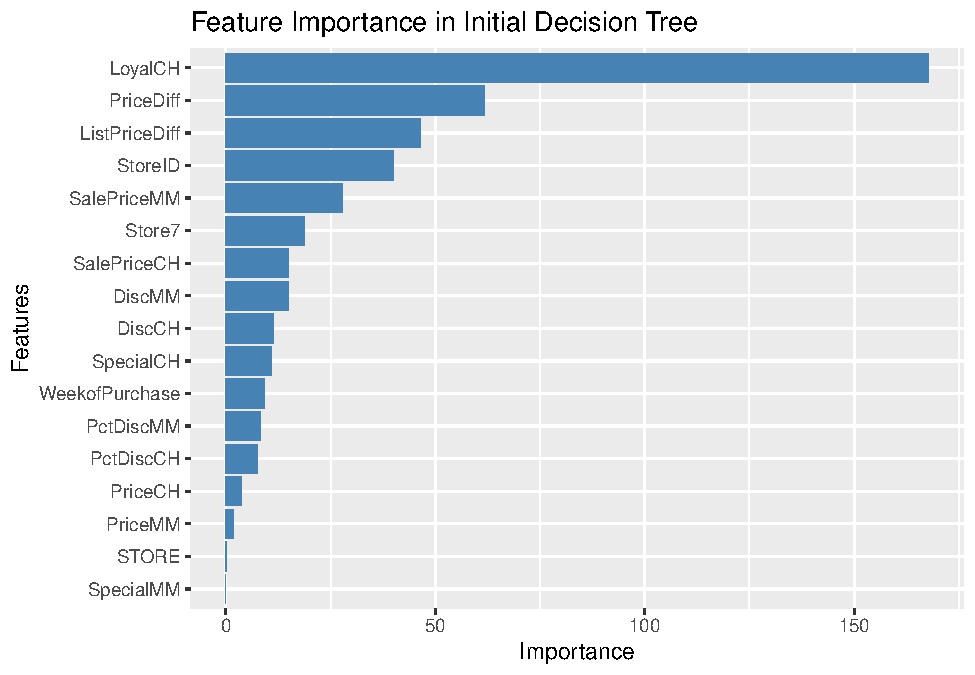
\includegraphics{OJ_files/figure-latex/unnamed-chunk-9-1.pdf}

This feature importance plot shows which variables contributed the most
to the Decision Tree splits. Variables with higher importance values
played a more significant role in determining whether a customer
purchased Citrus Hill or Minute Maid. This bar chart displays the
feature importance rankings from an initial decision tree model.
``LoyalCH'' has the highest importance, suggesting that customer loyalty
has the strongest impact on the model's predictions. Other key features,
such as ``PriceDiff'' and ``ListPriceDiff,'' also have significant
influence, while features like ``STORE'' and ``SpecialMM'' have minimal
impact, indicating they contribute less to the model's predictive power.

\hypertarget{improving-the-model-hyperparameter-tuning}{%
\subsection{Improving the Model: Hyperparameter
Tuning}\label{improving-the-model-hyperparameter-tuning}}

\begin{Shaded}
\begin{Highlighting}[]
\FunctionTok{set.seed}\NormalTok{(}\DecValTok{123}\NormalTok{)}
\NormalTok{tree\_tuned }\OtherTok{\textless{}{-}} \FunctionTok{train}\NormalTok{(Purchase }\SpecialCharTok{\textasciitilde{}}\NormalTok{ ., }\AttributeTok{data =}\NormalTok{ train\_data, }\AttributeTok{method =} \StringTok{"rpart"}\NormalTok{,}
                    \AttributeTok{trControl =} \FunctionTok{trainControl}\NormalTok{(}\AttributeTok{method =} \StringTok{"cv"}\NormalTok{, }\AttributeTok{number =} \DecValTok{10}\NormalTok{),}
                    \AttributeTok{tuneLength =} \DecValTok{10}\NormalTok{)}

\FunctionTok{plot}\NormalTok{(tree\_tuned)}
\end{Highlighting}
\end{Shaded}

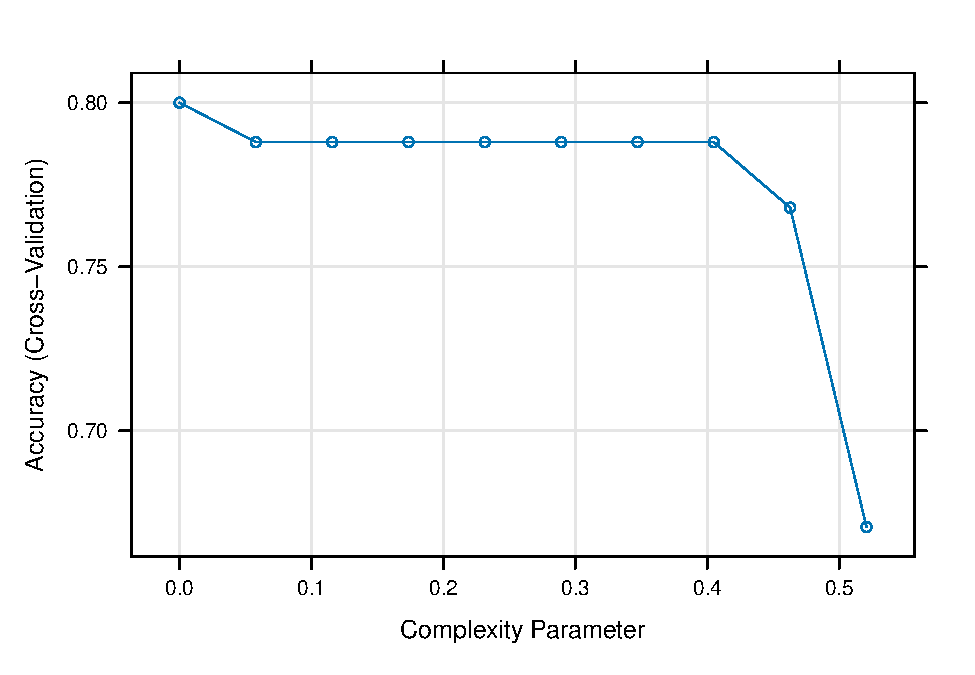
\includegraphics{OJ_files/figure-latex/unnamed-chunk-10-1.pdf}

We perform hyper parameter tuning using 10-fold cross-validation to find
the optimal complexity parameter (cp), which controls the depth and size
of the tree. Tuning prevents over fitting by balancing model complexity
and performance. This plot shows the relationship between the complexity
parameter and cross-validated accuracy for a model. As the complexity
parameter increases from 0 to around 0.4, accuracy remains relatively
stable, suggesting that adding complexity does not significantly improve
model performance. However, after 0.4, accuracy sharply declines,
indicating over fitting and that further complexity negatively impacts
the model's predictive power.

\hypertarget{final-decision-tree-and-evaluation}{%
\subsection{Final Decision Tree and
Evaluation}\label{final-decision-tree-and-evaluation}}

\begin{Shaded}
\begin{Highlighting}[]
\NormalTok{final\_tree\_model }\OtherTok{\textless{}{-}} \FunctionTok{rpart}\NormalTok{(Purchase }\SpecialCharTok{\textasciitilde{}}\NormalTok{ ., }\AttributeTok{data =}\NormalTok{ train\_data, }\AttributeTok{method =} \StringTok{"class"}\NormalTok{, }
                          \AttributeTok{control =} \FunctionTok{rpart.control}\NormalTok{(}\AttributeTok{cp =}\NormalTok{ tree\_tuned}\SpecialCharTok{$}\NormalTok{bestTune}\SpecialCharTok{$}\NormalTok{cp))}

\FunctionTok{rpart.plot}\NormalTok{(final\_tree\_model, }\AttributeTok{type =} \DecValTok{3}\NormalTok{, }\AttributeTok{extra =} \DecValTok{102}\NormalTok{, }\AttributeTok{under =} \ConstantTok{TRUE}\NormalTok{, }\AttributeTok{fallen.leaves =} \ConstantTok{TRUE}\NormalTok{,}
           \AttributeTok{main =} \StringTok{"Improved Decision Tree"}\NormalTok{)}
\end{Highlighting}
\end{Shaded}

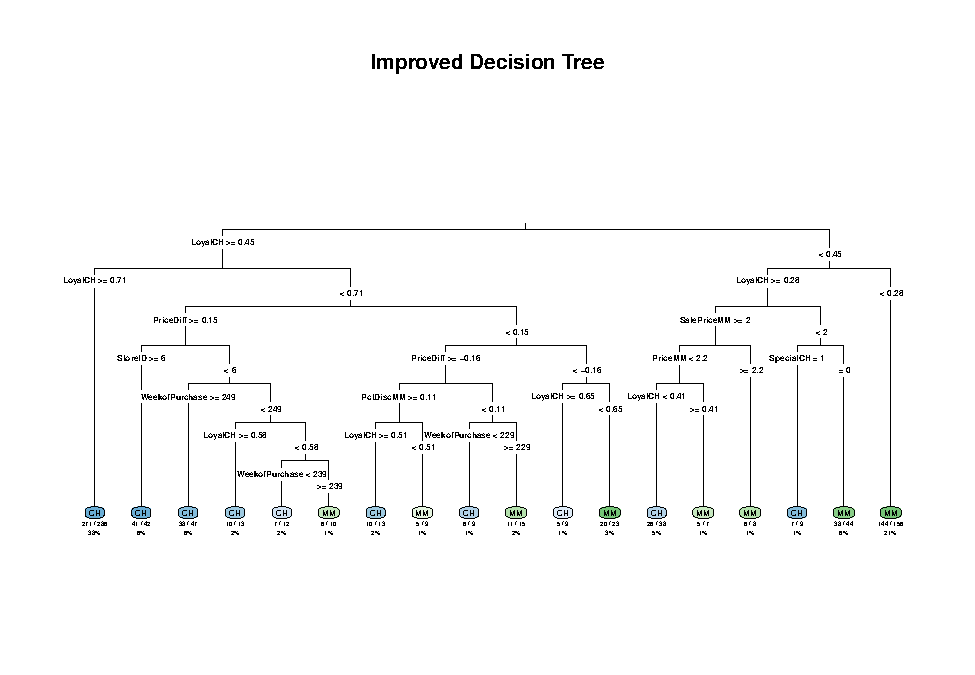
\includegraphics{OJ_files/figure-latex/unnamed-chunk-11-1.pdf}

This improved decision tree classifies customers into two categories,
``CH'' and ``MM,'' based on several factors, with \texttt{LoyalCH} (a
loyalty score) as the primary decision criterion. At the top level, if
\texttt{LoyalCH} is 0.45 or higher, the tree follows the left branch; if
it's lower, it goes right. For customers with \texttt{LoyalCH} above
0.71, further splits occur based on \texttt{PriceDiff} (price
difference), \texttt{StoreID}, and \texttt{WeekofPurchase} to classify
them as either ``CH'' or ``MM.'' If \texttt{LoyalCH} is between 0.45 and
0.71, additional checks on \texttt{PriceMM}, \texttt{PctDiscMM}, and
\texttt{WeekofPurchase} refine the classification. On the right side of
the tree, for those with \texttt{LoyalCH} below 0.45, decisions rely on
lower \texttt{LoyalCH} thresholds and other conditions like
\texttt{SalePriceMM} and \texttt{SpecialCH}, leading to final
classifications. The tree's added decision points on factors such as
\texttt{StoreID} and \texttt{WeekofPurchase} enhance its accuracy by
capturing store-specific and timing-based patterns, making it more
nuanced and effective in distinguishing between customer types.

\begin{Shaded}
\begin{Highlighting}[]
\NormalTok{final\_test\_pred }\OtherTok{\textless{}{-}} \FunctionTok{predict}\NormalTok{(final\_tree\_model, }\AttributeTok{newdata =}\NormalTok{ test\_data, }\AttributeTok{type =} \StringTok{"class"}\NormalTok{)}
\FunctionTok{confusionMatrix}\NormalTok{(final\_test\_pred, test\_data}\SpecialCharTok{$}\NormalTok{Purchase)}
\end{Highlighting}
\end{Shaded}

\begin{verbatim}
## Confusion Matrix and Statistics
## 
##           Reference
## Prediction  CH  MM
##         CH 165  31
##         MM  30  94
##                                          
##                Accuracy : 0.8094         
##                  95% CI : (0.762, 0.8509)
##     No Information Rate : 0.6094         
##     P-Value [Acc > NIR] : 1.07e-14       
##                                          
##                   Kappa : 0.599          
##                                          
##  Mcnemar's Test P-Value : 1              
##                                          
##             Sensitivity : 0.8462         
##             Specificity : 0.7520         
##          Pos Pred Value : 0.8418         
##          Neg Pred Value : 0.7581         
##              Prevalence : 0.6094         
##          Detection Rate : 0.5156         
##    Detection Prevalence : 0.6125         
##       Balanced Accuracy : 0.7991         
##                                          
##        'Positive' Class : CH             
## 
\end{verbatim}

\begin{Shaded}
\begin{Highlighting}[]
\NormalTok{final\_accuracy }\OtherTok{\textless{}{-}} \FunctionTok{sum}\NormalTok{(final\_test\_pred }\SpecialCharTok{==}\NormalTok{ test\_data}\SpecialCharTok{$}\NormalTok{Purchase) }\SpecialCharTok{/} \FunctionTok{nrow}\NormalTok{(test\_data)}
\FunctionTok{print}\NormalTok{(}\FunctionTok{paste}\NormalTok{(}\StringTok{"Final Accuracy:"}\NormalTok{, }\FunctionTok{round}\NormalTok{(final\_accuracy }\SpecialCharTok{*} \DecValTok{100}\NormalTok{, }\DecValTok{2}\NormalTok{), }\StringTok{"\%"}\NormalTok{))}
\end{Highlighting}
\end{Shaded}

\begin{verbatim}
## [1] "Final Accuracy: 80.94 %"
\end{verbatim}

We rebuild the Decision Tree using the optimal cp value found through
tuning. The new tree is expected to generalize better and prevent
overfitting. The final accuracy is 80.94\%, which is slightly lower than
the initial accuracy, but the model is now more robust and less likely
to overfit.

\hypertarget{confusion-matrix-and-performance-metrics}{%
\subsubsection{Confusion Matrix and Performance
Metrics}\label{confusion-matrix-and-performance-metrics}}

\hypertarget{confusion-matrix-overview-1}{%
\paragraph{\texorpdfstring{1. \textbf{Confusion Matrix
Overview}}{1. Confusion Matrix Overview}}\label{confusion-matrix-overview-1}}

\begin{itemize}
\item
  \textbf{Structure}:

  \begin{longtable}[]{@{}lll@{}}
  \toprule\noalign{}
  & Reference CH & Reference MM \\
  \midrule\noalign{}
  \endhead
  \bottomrule\noalign{}
  \endlastfoot
  \textbf{Predicted CH} & 165 & 31 \\
  \textbf{Predicted MM} & 30 & 94 \\
  \end{longtable}
\item
  \textbf{Interpretation}:

  \begin{itemize}
  \tightlist
  \item
    \textbf{True Positives (TP)}: 165 correctly predicted as CH.
  \item
    \textbf{False Negatives (FN)}: 31 incorrectly predicted as MM
    (actual CH).
  \item
    \textbf{False Positives (FP)}: 30 incorrectly predicted as CH
    (actual MM).
  \item
    \textbf{True Negatives (TN)}: 94 correctly predicted as MM.
  \end{itemize}
\end{itemize}

\hypertarget{model-performance-metrics-1}{%
\paragraph{\texorpdfstring{2. \textbf{Model Performance
Metrics}}{2. Model Performance Metrics}}\label{model-performance-metrics-1}}

\begin{itemize}
\tightlist
\item
  \textbf{Accuracy}: 80.94\% (correct predictions among total).
\item
  \textbf{95\% Confidence Interval (CI)}: (0.762, 0.8509) - true
  accuracy likely within this range.
\item
  \textbf{No Information Rate (NIR)}: 60.94\% - accuracy if only
  predicting the most frequent class.
\item
  \textbf{P-Value {[}Acc \textgreater{} NIR{]}}: 1.07e-14 - model
  significantly outperforms random guessing.
\end{itemize}

\hypertarget{kappa-statistic-1}{%
\paragraph{\texorpdfstring{3. \textbf{Kappa
Statistic}}{3. Kappa Statistic}}\label{kappa-statistic-1}}

\begin{itemize}
\tightlist
\item
  \textbf{Value}: 0.599 - indicates moderate agreement beyond chance.
\end{itemize}

\hypertarget{mcnemars-test-p-value-1}{%
\paragraph{\texorpdfstring{4. \textbf{Mcnemar's Test
P-Value}}{4. Mcnemar's Test P-Value}}\label{mcnemars-test-p-value-1}}

\begin{itemize}
\tightlist
\item
  \textbf{Value}: 1 - no significant difference in error rates for
  classes.
\end{itemize}

\hypertarget{sensitivity-true-positive-rate-1}{%
\paragraph{\texorpdfstring{5. \textbf{Sensitivity (True Positive
Rate)}}{5. Sensitivity (True Positive Rate)}}\label{sensitivity-true-positive-rate-1}}

\begin{itemize}
\tightlist
\item
  \textbf{Value}: 84.62\% - accurately identifies actual CH instances.
\end{itemize}

\hypertarget{specificity-true-negative-rate-1}{%
\paragraph{\texorpdfstring{6. \textbf{Specificity (True Negative
Rate)}}{6. Specificity (True Negative Rate)}}\label{specificity-true-negative-rate-1}}

\begin{itemize}
\tightlist
\item
  \textbf{Value}: 75.20\% - accurately identifies actual MM instances.
\end{itemize}

\hypertarget{positive-predictive-value-ppv-1}{%
\paragraph{\texorpdfstring{7. \textbf{Positive Predictive Value
(PPV)}}{7. Positive Predictive Value (PPV)}}\label{positive-predictive-value-ppv-1}}

\begin{itemize}
\tightlist
\item
  \textbf{Value}: 84.18\% - proportion of predicted CH that are actually
  CH.
\end{itemize}

\hypertarget{negative-predictive-value-npv-1}{%
\paragraph{\texorpdfstring{8. \textbf{Negative Predictive Value
(NPV)}}{8. Negative Predictive Value (NPV)}}\label{negative-predictive-value-npv-1}}

\begin{itemize}
\tightlist
\item
  \textbf{Value}: 75.81\% - proportion of predicted MM that are actually
  MM.
\end{itemize}

\hypertarget{prevalence-1}{%
\paragraph{\texorpdfstring{9.
\textbf{Prevalence}}{9. Prevalence}}\label{prevalence-1}}

\begin{itemize}
\tightlist
\item
  \textbf{Value}: 60.94\% - indicates the proportion of actual CH cases.
\end{itemize}

\hypertarget{detection-rate-1}{%
\paragraph{\texorpdfstring{10. \textbf{Detection
Rate}}{10. Detection Rate}}\label{detection-rate-1}}

\begin{itemize}
\tightlist
\item
  \textbf{Value}: 51.56\% - proportion of actual positives detected by
  the model.
\end{itemize}

\hypertarget{detection-prevalence-1}{%
\paragraph{\texorpdfstring{11. \textbf{Detection
Prevalence}}{11. Detection Prevalence}}\label{detection-prevalence-1}}

\begin{itemize}
\tightlist
\item
  \textbf{Value}: 61.25\% - proportion of instances predicted as CH.
\end{itemize}

\hypertarget{balanced-accuracy-1}{%
\paragraph{\texorpdfstring{12. \textbf{Balanced
Accuracy}}{12. Balanced Accuracy}}\label{balanced-accuracy-1}}

\begin{itemize}
\tightlist
\item
  \textbf{Value}: 79.91\% - average of sensitivity and specificity.
\end{itemize}

\hypertarget{positive-class-1}{%
\paragraph{\texorpdfstring{13. \textbf{Positive
Class}}{13. Positive Class}}\label{positive-class-1}}

\begin{itemize}
\tightlist
\item
  \textbf{Class Identified}: CH is considered the positive class for
  performance metrics.
\end{itemize}

\hypertarget{summary-1},
with a strong sensitivity of \textbf{84.62\%}, indicating that it
effectively identifies positive cases (CH). The model also performs well
in terms of specificity (\textbf{75.20\%}) and Kappa statistic
(\textbf{0.599}), which suggests a moderate level of agreement beyond
chance. The confidence interval and P-values indicate that the model's
performance is statistically significant and that it performs better
than random guessing. Overall, Model 2 demonstrates reliable predictive
capability for the task at hand. This Model demonstrates reliable
predictive capability for identifying the positive class (CH).

\hypertarget{comparative-analysis-of-model-performance}{%
\section{Comparative Analysis of Model
Performance}\label{comparative-analysis-of-model-performance}}

\hypertarget{model-1-metrics-before-cross-validation}{%
\subsection{Model 1 Metrics (Before
Cross-validation)}\label{model-1-metrics-before-cross-validation}}

\begin{itemize}
\tightlist
\item
  \textbf{Accuracy}: 81.56\%
\item
  \textbf{Sensitivity (True Positive Rate)}: 86.67\%
\item
  \textbf{Specificity (True Negative Rate)}: 73.60\%
\item
  \textbf{Positive Predictive Value (PPV)}: 83.66\%
\item
  \textbf{Negative Predictive Value (NPV)}: 77.97\%
\item
  \textbf{Kappa Statistic}: 0.6088
\item
  \textbf{Balanced Accuracy}: 80.13\%
\item
  \textbf{95\% Confidence Interval (CI)}: (0.7687, 0.8566)
\end{itemize}

\hypertarget{model-2-metrics-after-cross-validation}{%
\subsection{Model 2 Metrics (After
Cross-validation)}\label{model-2-metrics-after-cross-validation}}

\begin{itemize}
\tightlist
\item
  \textbf{Accuracy}: 80.94\%
\item
  \textbf{Sensitivity (True Positive Rate)}: 84.62\%
\item
  \textbf{Specificity (True Negative Rate)}: 75.20\%
\item
  \textbf{Positive Predictive Value (PPV)}: 84.18\%
\item
  \textbf{Negative Predictive Value (NPV)}: 75.81\%
\item
  \textbf{Kappa Statistic}: 0.599
\item
  \textbf{Balanced Accuracy}: 79.91\%
\item
  \textbf{95\% Confidence Interval (CI)}: (0.762, 0.8509)
\end{itemize}

\hypertarget{key-comparisons}{%
\subsection{Key Comparisons}\label{key-comparisons}}

\begin{enumerate}
\def\labelenumi{\arabic{enumi}.}
\tightlist
\item
  \textbf{Accuracy}: Model 1 has a slightly higher accuracy (81.56\%)
  compared to Model 2 (80.94\%).
\item
  \textbf{Sensitivity}: Model 1 also outperforms Model 2 in sensitivity
  (86.67\% vs.~84.62\%), indicating it is better at identifying actual
  positive cases (CH).
\item
  \textbf{Specificity}: Model 2 has a higher specificity (75.20\%
  vs.~73.60\%), meaning it is slightly better at identifying actual
  negative cases (MM).
\item
  \textbf{Positive Predictive Value (PPV)}: Model 2 performs better in
  terms of PPV (84.18\% vs.~83.66\%), suggesting it is more reliable
  when predicting CH instances.
\item
  \textbf{Negative Predictive Value (NPV)}: Model 1 has a better NPV
  (77.97\% vs.~75.81\%), indicating it is more effective at predicting
  negative instances.
\item
  \textbf{Kappa Statistic}: Model 1 shows a marginally better Kappa
  statistic (0.6088 vs.~0.599), indicating slightly stronger agreement
  beyond chance.
\item
  \textbf{Balanced Accuracy}: Model 1 has a better balanced accuracy
  (80.13\% vs.~79.91\%), highlighting a more favorable performance
  considering both classes.
\item
  \textbf{Confidence Intervals}: Both models show overlapping confidence
  intervals, but Model 1's is slightly higher, reinforcing its
  reliability.
\end{enumerate}

\hypertarget{conclusion}{%
\subsection{Conclusion}\label{conclusion}}

Both models demonstrate effective performance in predicting the
classification of instances as CH or MM. Model 1 (Before
Cross-validation) exhibits superior overall accuracy, sensitivity, and
negative predictive value, making it particularly strong in correctly
identifying actual positive cases and minimizing false negatives.
Conversely, Model 2 (After Cross-validation) shows a higher specificity
and positive predictive value, suggesting it is more reliable for
confirming negative cases.

In terms of general applicability, \textbf{Model 1 is recommended for
scenarios where accurately identifying positive cases is critical},
while \textbf{Model 2 may be preferable in contexts where correctly
predicting negative instances is more important}. Ultimately, the choice
between models should consider the specific requirements of the
application, particularly the costs associated with false positives and
false negatives.

In this analysis, I learned that evaluating model performance metrics
such as accuracy, sensitivity, and specificity is crucial for
understanding how well a model predicts outcomes. The comparison of two
models highlighted the importance of selecting the right model based on
the specific needs of the application, particularly in terms of false
positive and false negative rates. Ultimately, these insights will guide
my future work in model selection and performance evaluation.

\end{document}
